\documentclass{article}

\usepackage[margin=1.0in]{geometry}
\usepackage{graphicx}
\usepackage{amsmath}
\usepackage{float}
\usepackage{enumitem}
\usepackage{gensymb}

\title{CSC 577 HW2}
\date{1/23/2019}
\author{Simon Swenson}

\begin{document}

\pagenumbering{gobble}
\maketitle
\pagenumbering{arabic}

\section{Introduction}

This assignment was divided into two main sections, one focusing on model fitting 
and one focusing on reasoning about perspective in images. In the model fitting 
section, the focus was a comparison between non-homogeneous linear least squares 
fitting, using the now-familiar "dagger" of the input matrix, which we also explored 
in assignment 2, and a new method which treats the y coordinates of the input 
points equally to the x coordinates, which the non-homogeneous method did not 
use. In the image perspective system, we explore drawing parallel lines and 
making a judgment based on rules, namely, (1) that parallel lines in 3-d space 
lead to the same vanishing point in camera projection space and (2) that 
coplanar lines lead to the same horizon line. In the writeup, I use $\Theta$ to 
stand for the model parameters to prevent confusion with $X$ (input points). As 
always, latex tends to float figures around in strange ways, so please check 
adjacent pages whenever figures are referenced or where you expect a figure to 
appear. All questions for the assignment were completed.

\section{A Comparison of Line Fitting Strategies}

We are given an arbitrary set of 2-d points and asked to find a good line fit 
to that set. However, there are many different ways to fit a line. For this 
assignment, we just explored two: non-homogeneous least squares and 
homogeneous least squares. The main difference between the two formulations is 
that the first formulation treats the y axis (and the y coordinates of the input 
points) as completely different from the x axis (and x coordinates). In this 
formulation, error is only minimized vertically from each point to the regression 
line. In the second, error is minimized by the tangent of the regression line 
from each point to the regression line.

In the first formulation, we found that the least squares error was minimized 
by the following solution. (Note that I used $\Theta$ for model parameters.) Let 
$U = [X | 1]$. Then the solution is:

$$
\Theta = (U^T U)^{-1} U^T y
$$

In the second formulation, we found that the least squares error was minimized 
by letting the model parameters (a, b) equal the elements of the eigenvector 
with the smallest eigenvalue of $U^T U$, where 

$$
U = \begin{bmatrix}
x_1 - \bar{x} & y_1 - \bar{y} \\
x_2 - \bar{x} & y_2 - \bar{y} \\
\vdots        & \vdots \\
x_N - \bar{x} & y_N - \bar{y}
\end{bmatrix}
$$

Note that, in this formulation, the columns of $U$ are interchangeable. Thus, 
both x and y are treated the same. This is the key of the homogeneous least 
squares solution.

\begin{figure}[!ht]
	\centering
	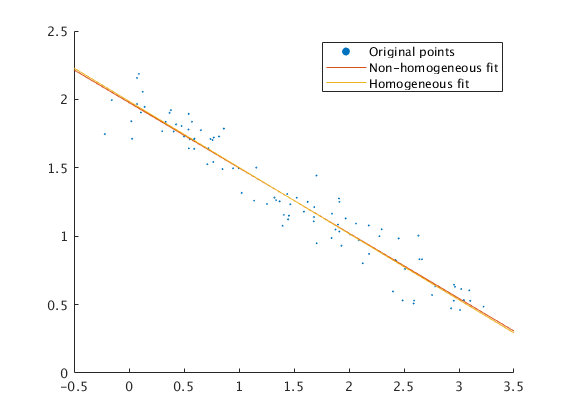
\includegraphics[width=120mm]{figs/line_fits.png}
	\caption{The original data points as a scatter plot, alongside both line 
        fits. You can see from the figure that both line fits are very similar, 
        but they are different, highlighting that each formulation leads to a 
        different result.}
\end{figure}

To compare the two models, we must come up with some way to convert the model 
parameters of one to the model parameters of the other. In other words, we must 
be able to convert a, b to slope, intercept and vise versa. For the first, we 
start with the equation:

$$
[X | Y] \begin{bmatrix}
a \\
b
\end{bmatrix} = \overrightarrow{0}
$$

Then we have:

\begin{align*}
\begin{bmatrix}
x_1 - \bar{x} & y_1 - \bar{y} \\
x_2 - \bar{x} & y_2 - \bar{y} \\
\vdots        & \vdots        \\
x_N - \bar{x} & y_N - \bar{y} \\
\end{bmatrix} \begin{bmatrix}
a \\
b
\end{bmatrix} &= \overrightarrow{0} \\
\begin{bmatrix}
(x_1 - \bar{x})a + (y_1 - \bar{y})b \\
(x_2 - \bar{x})a + (y_2 - \bar{y})b \\
\vdots \\
(x_N - \bar{x})a + (y_N - \bar{y})b \\
\end{bmatrix} &= \overrightarrow{0} \\
a \begin{bmatrix}
x_1 - \bar{x} \\
x_2 - \bar{x} \\
\vdots \\
x_N - \bar{x} \\
\end{bmatrix} &= -b \begin{bmatrix}
y_1 - \bar{y} \\
y_2 - \bar{y} \\
\vdots \\
y_N - \bar{y} \\
\end{bmatrix} \\
-\frac{a}{b} \begin{bmatrix}
x_1 - \bar{x} \\
x_2 - \bar{x} \\
\vdots \\
x_N - \bar{x} \\
\end{bmatrix} &= \begin{bmatrix}
y_1 - \bar{y} \\
y_2 - \bar{y} \\
\vdots \\
y_N - \bar{y} \\
\end{bmatrix} \\
\end{align*}
% Have to split here, or the equations were running off the end of the screen.
\begin{align*}
-\frac{a}{b} (\begin{bmatrix}
x_1 \\
x_2 \\
\vdots \\
x_N \\
\end{bmatrix} - \bar{x})&= \begin{bmatrix}
y_1 \\
y_2 \\
\vdots \\
y_N \\
\end{bmatrix} - \bar{y} \\
-\frac{a}{b} \begin{bmatrix}
x_1 \\
x_2 \\
\vdots \\
x_N \\
\end{bmatrix} + \frac{\bar{x} a}{b} &= \begin{bmatrix}
y_1 \\
y_2 \\
\vdots \\
y_N \\
\end{bmatrix} - \bar{y} \\
-\frac{a}{b} \begin{bmatrix}
x_1 \\
x_2 \\
\vdots \\
x_N \\
\end{bmatrix} + \frac{\bar{x} a}{b} + \bar{y} &= \begin{bmatrix}
y_1 \\
y_2 \\
\vdots \\
y_N \\
\end{bmatrix} \\
\begin{bmatrix}
x_1 & 1 \\
x_2 & 1 \\
\vdots & \vdots \\
x_N & 1 \\
\end{bmatrix} \begin{bmatrix}
-\frac{a}{b} \\
\frac{\bar{x} a}{b} + \bar{y} \\
\end{bmatrix} &= \begin{bmatrix}
y_1 \\
y_2 \\
\vdots \\
y_N \\
\end{bmatrix} \\
\end{align*}

In this form, it is clear that $m = -\frac{a}{b}$ and $b = \frac{\bar{x} a}{b} + \bar{y}$. 
Now, to convert in the other direction, we use the following equations, solving 
for a, b:

\begin{align*}
m = -\frac{a}{b} \\
a^2 + b^2 = 1
\end{align*}

First, we solve for a in the first equation:

$$
a = -m b
$$

Then, we substitute that $a$ into the second equation:

\begin{align*}
(-m b)^2 + b^2 &= 1 \\
m^2 b^2 + b^2 &= 1 \\
b^2 (m^2 + 1) &= 1 \\
b^2 = \frac{1}{m^2 + 1} \\
b = \pm \sqrt{\frac{1}{m^2 + 1}}
\end{align*}

Finally, we plug that b into the first equation:

$$
a = -m \pm \sqrt{\frac{1}{m^2 + 1}}
$$

Now that we have a method to convert each model into the other, we can gather 
some results:

\begin{tabular}{r | r r}
                         & Non-homogeneous Model & Homogeneous Model \\
          Slope          &         -0.4772       &           -0.4840 \\
    Y-intercept          &          1.9769       &            1.9868 \\
              A          &          0.4307       &           -0.4357 \\
              B          &          0.9025       &           -0.9001 \\
    Non-homogeneous RMSE &          0.1250       &            0.1252 \\
        Homogeneous RMSE &          0.1128       &            0.1127 \\
\end{tabular}

We see from the results that both models have a higher non-homogeneous RMSE than 
homogeneous RMSE. The following figure attempts to explain why that is the case:

\begin{figure}[!ht]
	\centering
	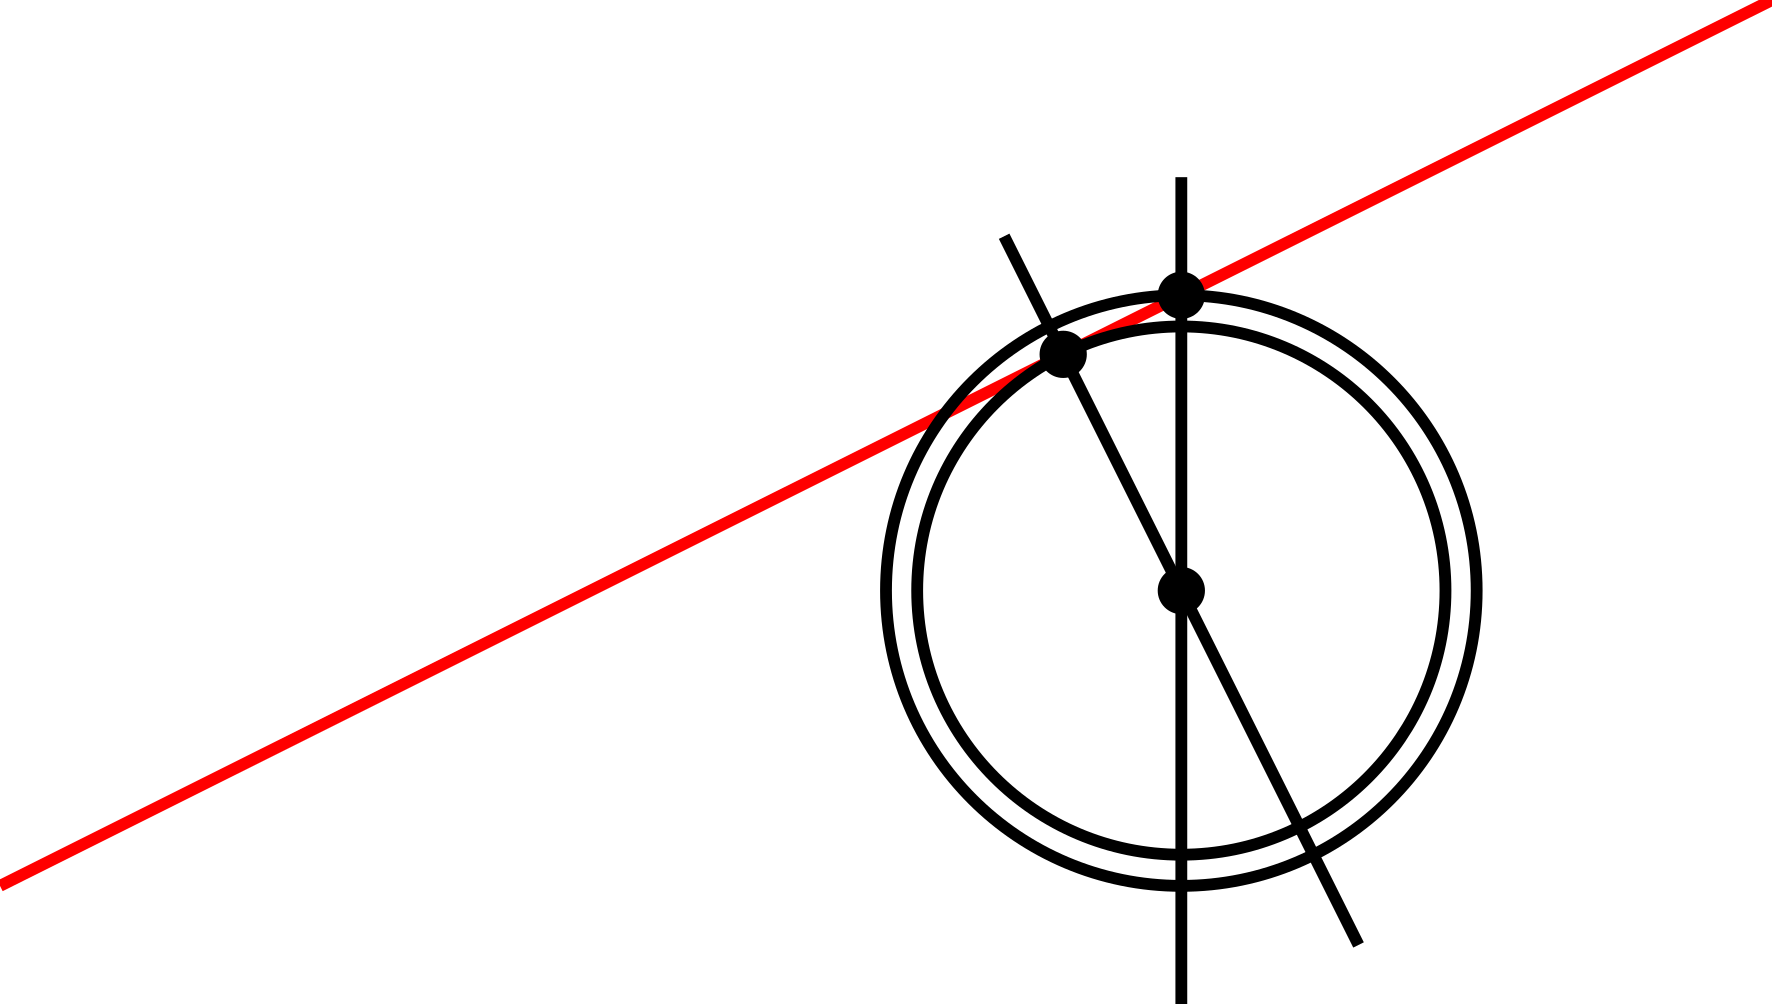
\includegraphics[width=120mm]{figs/error_comparison.png}
	\caption{A diagram illustrating non-homogeneous error (vertical distance) 
        and homogeneous error (tangent distance). Notice that the homogeneous 
        error is less. (Compare the circle radii.) In fact, this is the case for 
        all fits, save for a horizontal line.}
\end{figure}

Now that we have explored the relationship between the two error metrics, let's 
explore the relationship between each error metric and both models. As we 
discussed in class, the non-homogeneous solution minimizes the mean squared 
error. Thus, we would expect any other solution, even the homogeneous solution, 
to have a higher non-homogeneous RMSE. This is indeed the case. A similar 
situation arises for homogeneous RMSE. We know by derivation that the 
homogeneous model will minimize the homogeneous mean squared error, and we can 
indeed see that that is the case based on our results.

\section{Line Fitting - Graduate Discussion}

Our observations above can be formalized below.

\subsection{Theorem: Homogeneous MSE will always be less than or equal to non-homogeneous MSE}

For a geometric proof sketch, refer to the nearby diagram (showing circles 
representing absolute distance). Since squared distance as a function of 
absolute distance is monotonically increasing (consider the right-hand side of a 
parabola), the diagram holds for squared distance as well as absolute distance. 
Thus, it applies to mean squared error. The diagram also holds for any angle of 
line and any data point offset. (When the line is horizontal, homogeneous MSE 
equals non-homogeneous MSE, but because of how we've stated the theorem, the 
theorem still holds.)

\subsection{Theorem: The non-homogeneous model given above ensures a non-homogeneous error less than or equal to any possible linear model}

When discussing minimum values, it is always a good idea to turn to the idea of 
derivatives. Doing derivatives in vector space is a bit tricky, however. We turn 
to the idea of the gradient, which uses derivatives in the form of a vector. The 
gradient is a vector that always points in the direction of greatest 
positive change. Note that, at a peak (maximum) or valley (minimum), there is no 
direction of greatest positive change, so the gradient is 0. Recall that the 
gradient is defined as:

$$
grad(f(m, b)) = \begin{bmatrix}
\frac{\delta f}{\delta m} \\
\frac{\delta f}{\delta b}
\end{bmatrix}
$$

Note that we treat m and b as unknowns in this formulation: We flip the roles of 
the data-points (X, y) and the model parameters when we "train." (Although I am 
being a bit loose with the word "train" in this scenario.)

Let us return to the original error formulation and apply the gradient in terms 
of m and b:

$$
homogeneous\_mse = \frac{\sum_{1..N} (x_i m + b - y_i)^2}{N}
$$

Then:

\begin{align*}
grad(homogeneous\_mse) &= \begin{bmatrix}
\frac{\delta homogeneous\_mse}{\delta m} \\
\frac{\delta homogeneous\_mse}{\delta b}
\end{bmatrix}\\
&= \begin{bmatrix}
\frac{\delta}{\delta m} (\frac{\sum_{1..N} (x_i m + b - y_i)^2}{N}) \\
\frac{\delta}{\delta b} (\frac{\sum_{1..N} (x_i m + b - y_i)^2}{N})
\end{bmatrix}
\end{align*}

Let's first consider the derivative wrt m:

$$
\frac{\delta homogeneous\_mse}{\delta m} = \frac{2}{N} \sum_{1..N} ((x_i m + b - y_i)x_i)
$$

Similarly, we figure the derivative wrt b:

$$
\frac{\delta homogeneous\_mse}{\delta b} = \frac{2}{N} \sum_{1..N} (x_i m + b - y_i)
$$

To find the extrema, we set the gradient to the zero vector and solve:

\begin{align*}
\overrightarrow{0} &= \frac{2}{N} \begin{bmatrix}
\sum_{1..N} ((x_i m + b - y_i)x_i)\\
\sum_{1..N} (x_i m + b - y_i)
\end{bmatrix} \\
\overrightarrow{0} &= \frac{2}{N} \sum_{1..N} \begin{bmatrix}
(x_i m + b - y_i)x_i \\
x_i m + b - y_i
\end{bmatrix} \\
\overrightarrow{0} &= \frac{2}{N} \sum_{1..N} \begin{bmatrix}
x_i^2 m + x_i b - x_i y_i \\
x_i m + b - y_i
\end{bmatrix} \\
\overrightarrow{0} &= \sum_{1..N} \begin{bmatrix}
x_i^2 m + x_i b \\
x_i m + b
\end{bmatrix} - \sum_{1..N} \begin{bmatrix}
x_i y_i \\
y_i
\end{bmatrix} \\
\sum_{1..N} \begin{bmatrix}
x_i y_i \\
y_i
\end{bmatrix} &= \sum_{1..N} \begin{bmatrix}
x_i^2 m + x_i b \\
x_i m + b
\end{bmatrix} \\
\sum_{1..N} \begin{bmatrix}
x_i y_i \\
y_i
\end{bmatrix} &= \sum_{1..N} \begin{bmatrix}
x_i^2 & x_i \\
x_i   & 1
\end{bmatrix} \begin{bmatrix}
m \\
b
\end{bmatrix} \\
\begin{bmatrix}
\sum_{1..N} x_i y_i \\
\sum_{1..N} y_i
\end{bmatrix} &= \begin{bmatrix}
\sum_{1..N} x_i^2 & \sum_{1..N} x_i \\
\sum_{1..N} x_i   & N
\end{bmatrix} \begin{bmatrix}
m \\
b
\end{bmatrix}
\end{align*}

From here, we use standard techniques to find the inverse matrix of the matrix 
on the right (which we are multiplying by (m, b) on the left). As the expression 
gets quite unmanageable otherwise, I will omit the subscripts for 
$ \sum, x, y $. They are assumed.

\begin{align*}
\frac{1}{N \sum x^2 - \sum x \sum x} \begin{bmatrix}
N        & - \sum x \\
- \sum x & \sum x^2
\end{bmatrix} \begin{bmatrix}
\sum x y \\
\sum y
\end{bmatrix} &= \frac{1}{N \sum x^2 - \sum x \sum x} \begin{bmatrix}
N        & - \sum x \\
- \sum x & \sum x^2
\end{bmatrix} \begin{bmatrix}
\sum x^2 & \sum x \\
\sum x   & N
\end{bmatrix} \begin{bmatrix}
m \\
b
\end{bmatrix}
\end{align*}
% Have to split here, or the equations were running off the end of the screen.
\begin{align*}
\frac{1}{N \sum x^2 - \sum x \sum x} \begin{bmatrix}
N        & - \sum x \\
- \sum x & \sum x^2
\end{bmatrix} \begin{bmatrix}
\sum x y \\
\sum y
\end{bmatrix} &= \begin{bmatrix}
m \\
b
\end{bmatrix}
\end{align*}

Now, we will attempt to derive the same expression from the formulation of the 
non-homogeneous solution presented in class:

\begin{align*}
\begin{bmatrix}
m \\
b
\end{bmatrix} &= (U^T U)^{-1} U^T Y
\end{align*}

We begin:

\begin{align*}
U &= 
\begin{bmatrix}
x_1    & 1 \\
x_2    & 1 \\
\vdots & \vdots \\
x_N    & 1 \\
\end{bmatrix} \\
U^T U &= \begin{bmatrix}
x_1 & x_2 & \cdots & x_N \\
1   & 1   & \cdots & 1
\end{bmatrix} \begin{bmatrix}
x_1    & 1 \\
x_2    & 1 \\
\vdots & \vdots \\
x_N    & 1 \\
\end{bmatrix} \\
&= \begin{bmatrix}
\sum x^2 & \sum x \\
\sum x   & N
\end{bmatrix} \\
(U^T U)^{-1} &= \frac{1}{N \sum x^2 - \sum x \sum x} \begin{bmatrix}
N        & - \sum x \\
- \sum x & \sum x^2
\end{bmatrix} \\ 
(U^T U)^{-1} U^T Y &= \frac{1}{N \sum x^2 - \sum x \sum x} \begin{bmatrix}
N        & - \sum x \\
- \sum x & \sum x^2
\end{bmatrix} \begin{bmatrix}
x_1 & x_2 & \cdots & x_N \\
1   & 1   & \cdots & 1
\end{bmatrix} \begin{bmatrix}
y_1 \\
y_2 \\
\vdots \\
y_N
\end{bmatrix} \\
&= \frac{1}{N \sum x^2 - \sum x \sum x} \begin{bmatrix}
N        & - \sum x \\
- \sum x & \sum x^2
\end{bmatrix} \begin{bmatrix}
\sum x y \\
\sum y
\end{bmatrix}
\end{align*}

The two expressions are the same, so it is thus proven.

Note: To complete the proof, we would need to verify that we have actually found a minimum 
based on concavity, but that's a bit tedious for this assignment, so I will 
leave it as is.

\subsection{Theorem: The homogeneous model given above ensures a homogeneous error less than or equal to any possible linear model}

The proof sketch follows from the optional material found in slide deck 5. We 
initially want to find x in the following:

$$
U x \approx \overrightarrow{0}
$$

with the constraint:

$$
|| x || = 1
$$

Note that the equation above has no exact solution, so we want to minimize 
$ U x $. Since $ U x $ is not square, we multiply on the left by the transpose, similar 
to how we handled the non-homogeneous solution. This expression is the squared 
error. Then we want to minimize:

$$
min(x^T U^T U x)
$$

with the constraint:

$$
x^T x = 1
$$

We can rewrite $U^T U$ based on its eigen decomposition. Then the expression 
above becomes:

$$
min(x^T V \Lambda V^T x)
$$

It can be shown that $ U^T U $ is symmetric. Furthermore, it can be shown that 
eigenvectors of symmetric matrices are orthogonal. Then the dot product between 
of those distinct eigenvectors is 0. If we let $x$ equal the eigenvector that 
corresponds to the smallest eigenvalue, $V^T x$ becomes a vector with one 1 and 
the remaining entries 0 because one 
entry is the dot product of a unit vector with itself and all other entries are the dot 
product between orthogonal vectors and are thus 0. Note that this is the case 
\textit{for any eigenvector that we choose}. A similar vector arises on the 
other side ($x^T V$). Thus, in this formulation, the only real thing we have 
control over is selecting 
which entry in $\Lambda$ that we select (by picking a different eigenvector). 
Obviously, we want the smallest, so we pick the eigenvector that corresponds to 
the smallest eigenvalue.

This is an argument for why, if we restrict our search 
to only eigenvectors, we should pick the eigenvector with the smallest 
eigenvalue, but why restrict our picks to the eigenvectors, in the first place? Why 
couldn't the solution be some other random unit vector? Well, it has to do with 
the way eigenvectors work. Building off of what we learned about PCA from a 
previous assignment, the eigenvector with the largest eigenvalue will point in 
the direction of maximum variance. For a roughly linear distribution, this 
is the same direction as the line, itself. However, we learned from class that 
$a, b$ is orthogonal to the line that we want. Knowing that eigenvectors of 
symmetric matrices are orthogonal, by process of elimination, we must pick the 
eigenvector with the smallest eigenvalue to be $a, b$.

\subsection{Discussion: What if our solution is just a local minimum?}

This is a familiar concept to anyone familiar with machine learning. Often, the 
error function does not have a single extremum. If our solution only gives a local 
minimum, we have no good way of knowing if that minimum is also a global 
minimum, assuming all minima cannot be solved for explicitly. (If we have the 
set of all minima, we can do calculations to find out which is the global 
minimum.) Often, the set of all minima cannot be solved for explicitly, in which 
case gradient descent over the error function is often used. Starting from an 
arbitrary point, we repeatedly walk in the opposite direction of the gradient 
of the error function until we reach a minima. Intuitively, since we are taking 
steps, the process only knows about the immediate surroundings of our current 
point. It doesn't know the layout of the entire error function. Thus, it is 
impossible to know if we've reached a global minimum after such a process.

\section{Reasoning About Perspective: Skyscraper}

This image is fairly easy to reason about because the skyscraper is a fairly 
regular object. Here, we can easily draw the first two sets of parallel lines: 
vertical along the front face and horizontal along the front face. 
The third set of points can be generated by 
counting windows (six windows heigher on the left-hand side than the right-hand 
side). All sets of lines do roughly meet at corresponding common points. In 
addition, we find that those points are all co-linear. Thus, we conclude that 
the image is in proper perspective.

\begin{figure}[!ht]
	\centering
	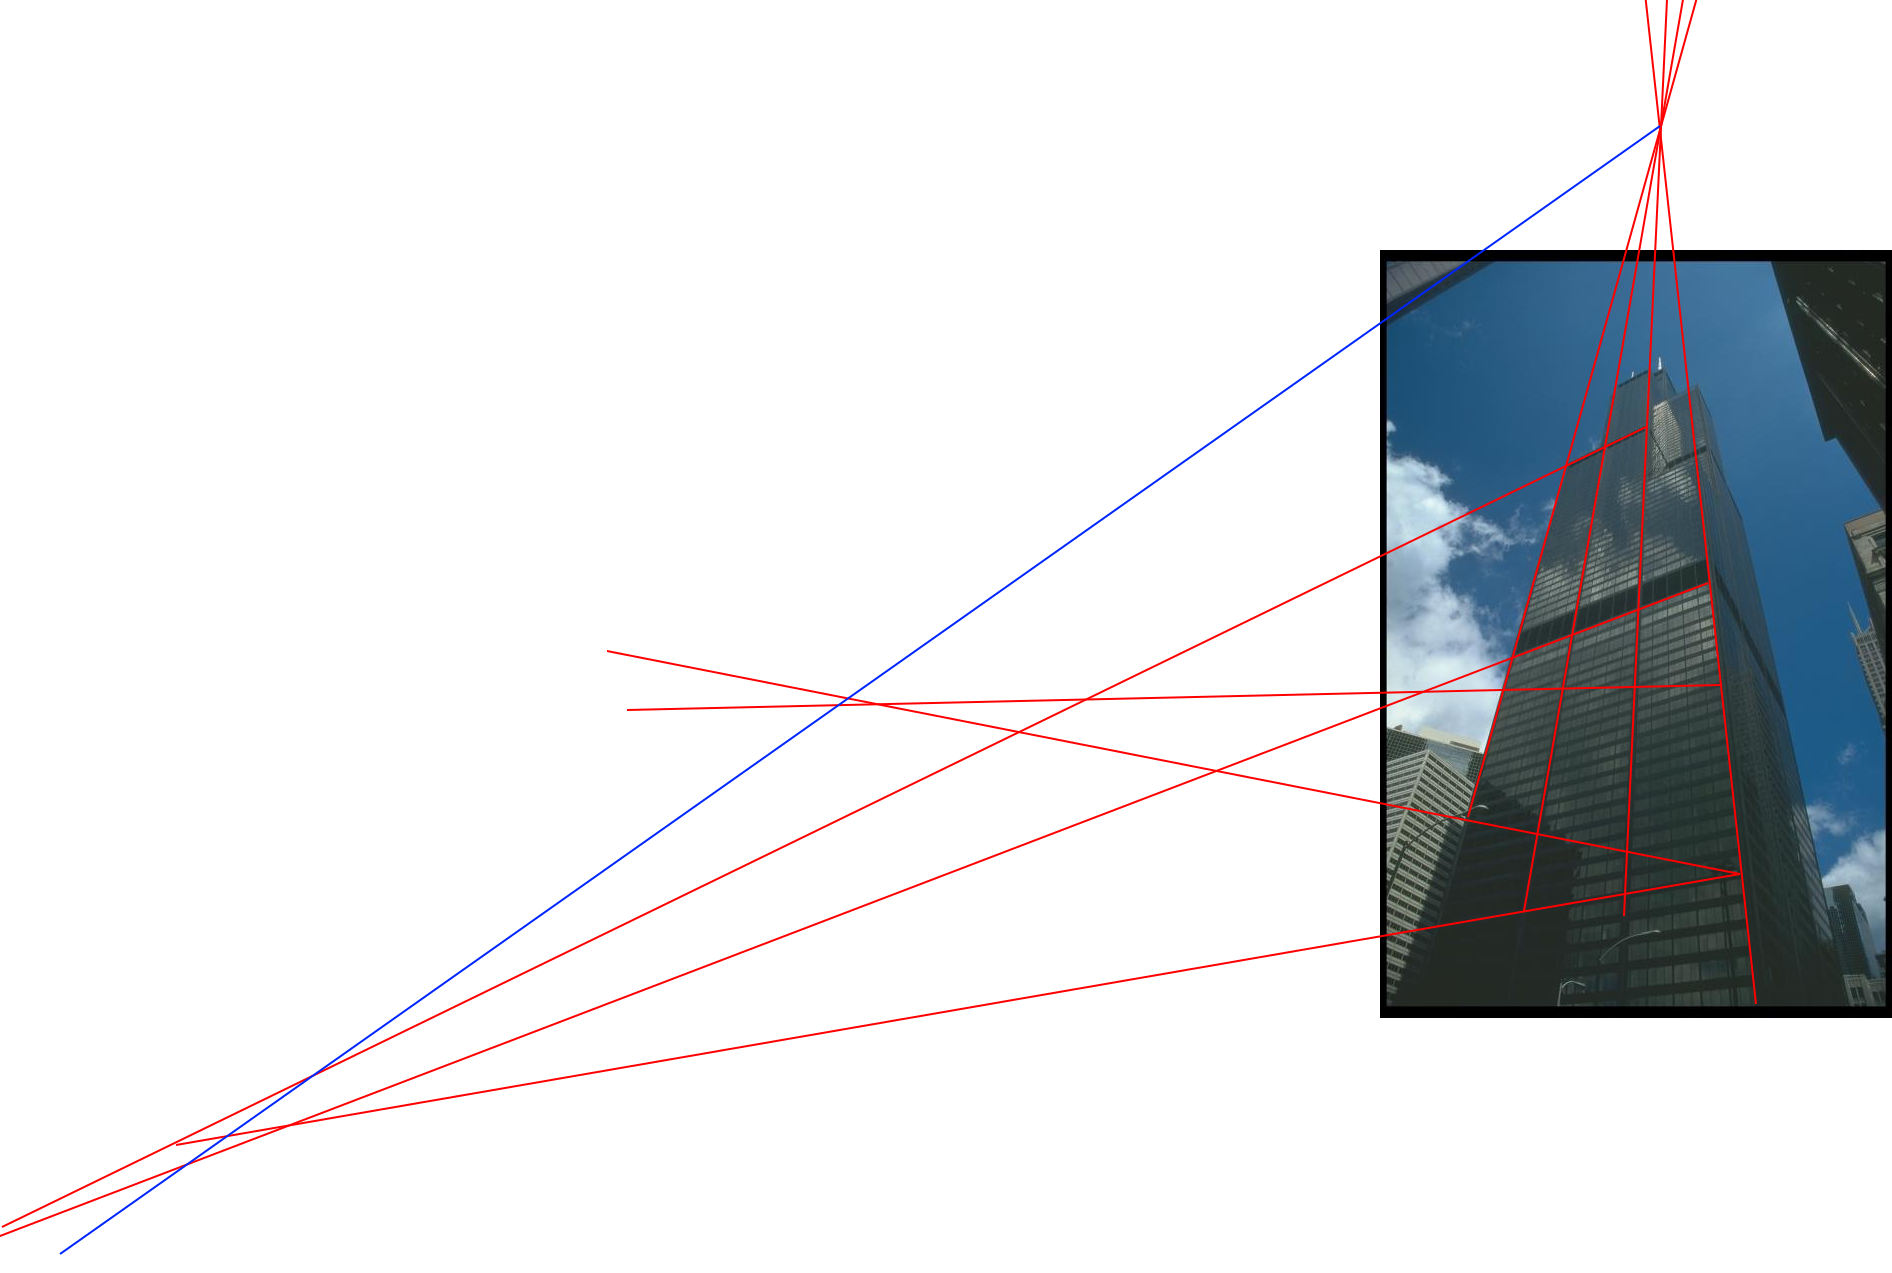
\includegraphics[width=160mm]{figs/building_lines.png}
	\caption{A skyscraper. By following parallel, coplanar 
        lines in world space, we find that parallel lines meet at common points 
        and sets of coplanar, parallel lines produce common points along a 
        common horizon line.}
\end{figure}

\section{Reasoning About Perspective: Chandelier}

The candels of this chandelier look to be aligned in a hexagon. If we assume 
that the hexagon is fairly regular, we can assume that the opposite edges are 
parallel in world coordinates. When we draw those corresponding lines, most do, 
indeed, meet at a point in projection space. However, one set does not. In 
addition, when we do this for all three pairs of parallel 
lines of the hexagon, we see that the three corresponding intersection points 
are not co-linear in projection space, which we would expect, since these points 
are all co-planar in world space. 
Thus, we can conclude that the image is \textit{not} in proper perspective.

\begin{figure}[!ht]
	\centering
	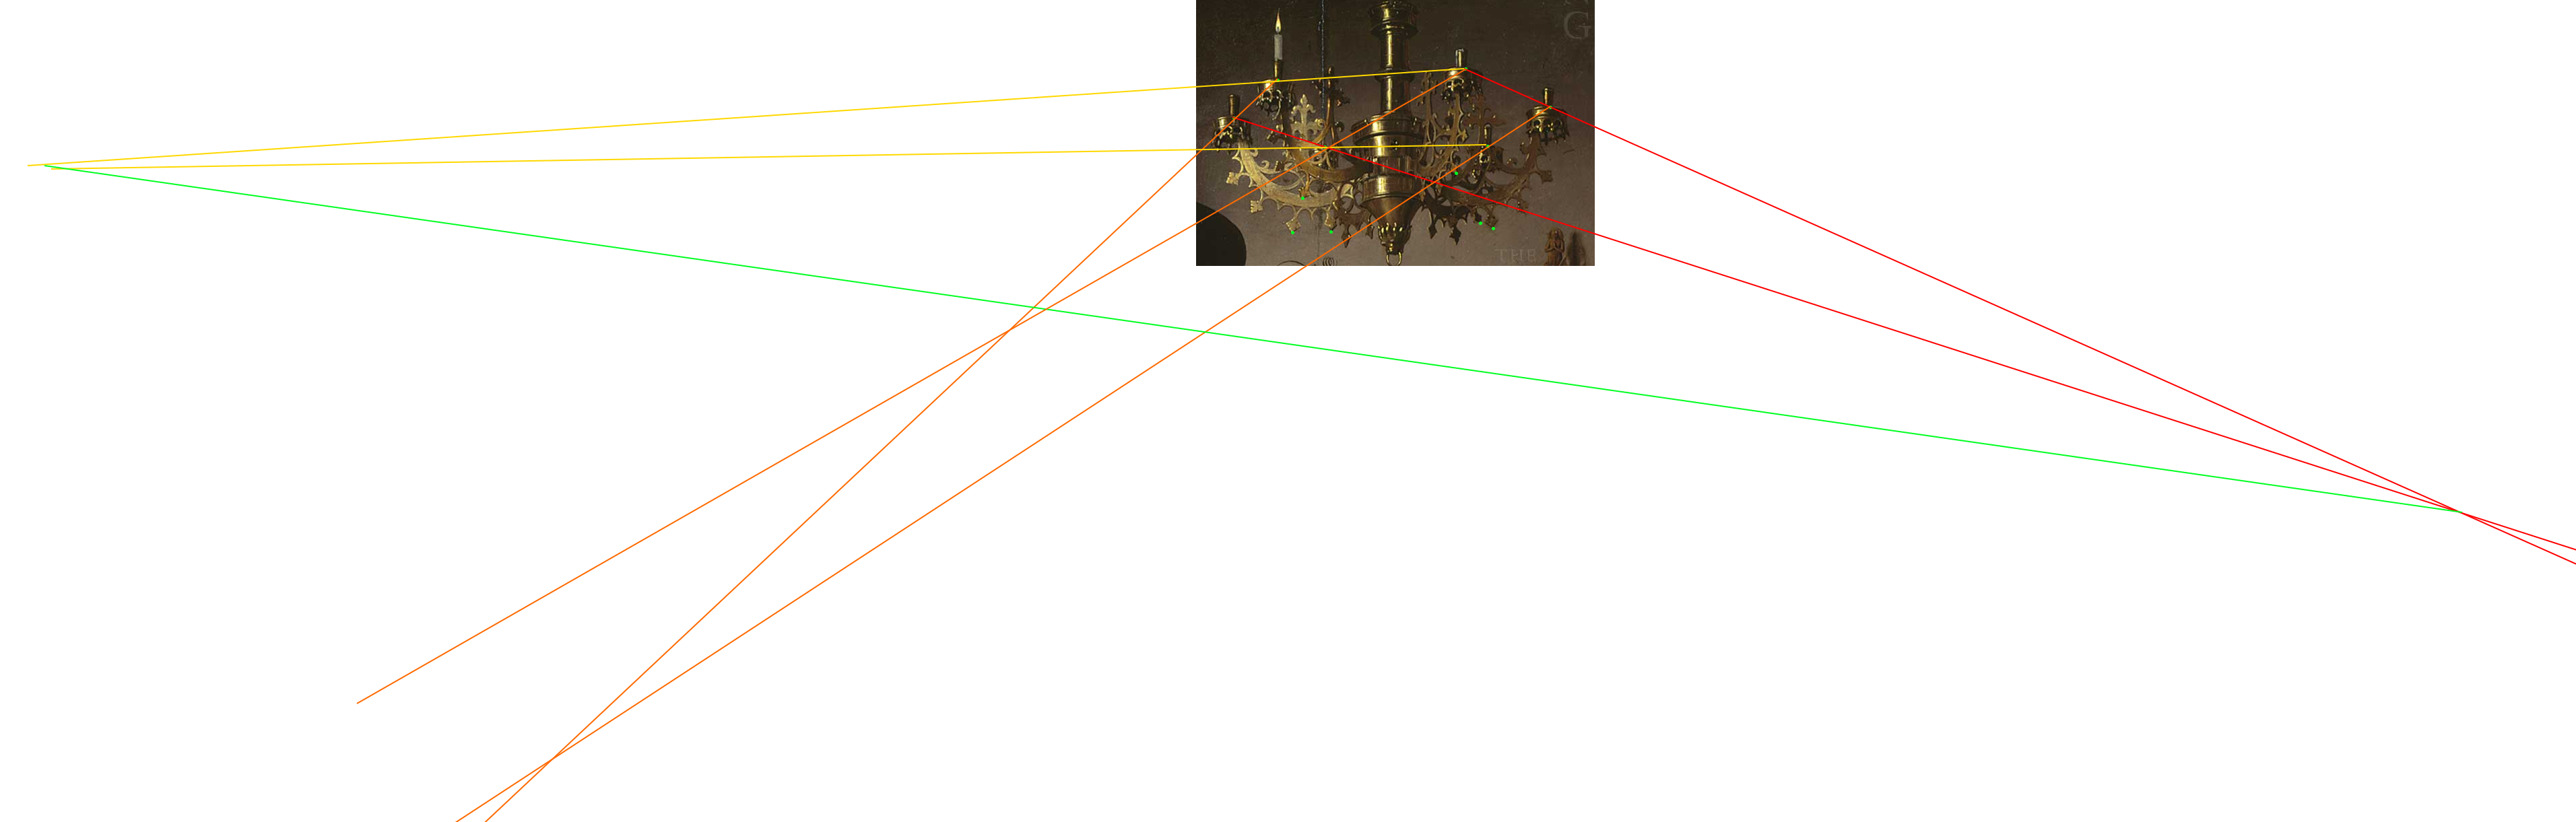
\includegraphics[width=160mm]{figs/chandelier_lines.png}
	\caption{A painting(?) of a chandelier. By following parallel, coplanar 
        lines in world space, we find that the resultant rays in projection 
        space are not co-linear.}
\end{figure}

\end{document}